\chapter[Resultados parciais]{Resultados parciais}\label{chap:resultados}


\section{Revisão sistemática}

A condução do processo de revisão sistemática pode ser entendida como uma abordagem em três fases como apresentado na Figura \ref{fig:fases_rs}.

\begin{figure}[!htb]
    \centering
    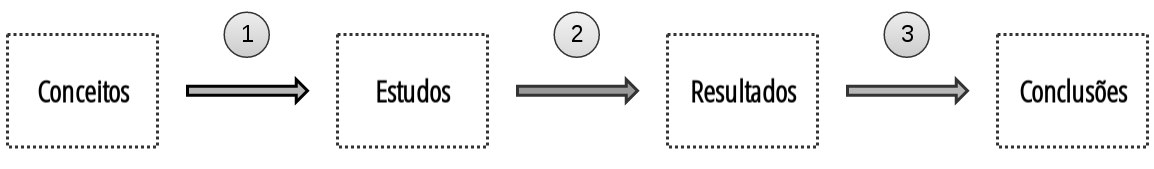
\includegraphics[scale=0.4]{figuras/fases_rs.png}    
    \caption{Abordagem de revisão sistemática em três fases. Traduzido. Fonte: \citeauthor{biolchini2005}, \citeyear{biolchini2005}.}
    \label{fig:fases_rs}
\end{figure}


A primeira fase da pesquisa começa a partir de conceitos, que de forma explícita e formalmente representam o assunto em questão. São definidos os procedimentos que pesquisador deve utilizar. Em seguida, é realizada a análse dos estudos que podem conter as informações e evidências sobre o tema específico da investigação \cite{biolchini2005}. 

A segunda fase começa a partir destes estudos coletados. Neste momento é realizada a distinção de quais estudos são relevantes e irrelevantes para o propósito da investigação. São examinados em seus conteúdos, comparados entre si, e às vezes reagrupados em suas partes. Obtêm-se assim os resultados, que representam o surgimento de um novo tipo de provas \cite{biolchini2005}. 

A terceira fase parte destes resultados. É realizado um processo de análise e síntese deste rearranjo de dados. E, por fim, chega-se às conclusões, que implicam em adquirir novos conhecimentos sobre o assunto em questão, bem como apoiar alguma decisão fazendo com ele relacionados \cite{biolchini2005}.





